% 17-18(본책 17쪽) — ㄴ자 모양 도로망(아래 가로 4칸·세로 1칸 띠 + 그 오른쪽 위로 가로 2칸·세로 3칸 블록). A 왼쪽 아래 · B 오른쪽 위. 스캔 그림을 TikZ 로 다시 그림(스캔 화질).
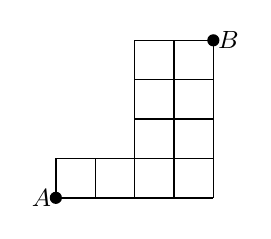
\begin{tikzpicture}[line width=0.5pt]
  % 아래 띠(가로 4칸·세로 1칸)
  \foreach \x in {0, 0.5, 1, 1.5, 2} { \draw (\x,0) -- (\x,0.5); }
  \foreach \y in {0, 0.5} { \draw (0,\y) -- (2,\y); }
  % 위 블록(가로 2칸·세로 3칸)
  \foreach \x in {1, 1.5, 2} { \draw (\x,0.5) -- (\x,2); }
  \foreach \y in {1, 1.5, 2} { \draw (1,\y) -- (2,\y); }
  \fill (0,0) circle (2.2pt);
  \node[left, font=\small, inner sep=1.5pt] at (0,0) {$\pt{A}$};
  \fill (2,2) circle (2.2pt);
  \node[right, font=\small, inner sep=1.5pt] at (2,2) {$\pt{B}$};
\end{tikzpicture}
